\chapter{Robotic Maintenance on Topside Offshore Platforms}
\label{chp:maintenance}

\section{Introduction}

This project is a small step towards a larger long-term goal concerning robotic maintenance on topside offshore installations. This chapter puts the implementation described in chapter \ref{chp:implementation}, into the context of the long-term goal. 

Over the last decade, the \ac{OG} industry has shown an increased interest in the potential benefits of automating the normal operation of remote offshore installations. Some satellite platforms, such as Sleipner B are already unmanned during normal operation, and the more recent Valemon platform is planned to become normally unmanned as well. It is now clear that robotics has several potential applications in process plants, and particularly in remote \ac{OG} installations. It is, however, difficult to predict how and to what extent robots will be applied in plant automation as other innovative solutions may arise\cite{statoil_ubemannet}\cite{subsea_konkurranse}\cite{E24}. Current research on plant automation is mainly motivated by two factors\cite{AutonomousOG} \cite{StepwiseApproachToRobotics}:

\begin{itemize}
	\item \textbf{HSE} - Reduced risk exposure for personnel and environment. 
	\item \textbf{Efficiency} - Accomplish more with less effort, resources and time. This means cost reduction by keeping downtime to a minimum with the least amount of effort.
\end{itemize} 

An additional overarching driving factor is that \ac{OG} fields are becoming more difficult to reach. As \ac{OG} fields in shallow waters are depleted, production is moved to deeper waters. This complicates the extraction process and reduces the profit margin. A solution to this challenge is to increase efficiency through further automation. 

This chapter provides a brief introduction to how topside maintenance is performed today, how these maintenance tasks could be robotized. The section is concluded with a discussion on how well modern robotics is suited for the task. 

%\subsection{Potential Maintenance Tasks}

%Hidden failure modes: PFD: What is the probability that a device (Fire detector, shut down valve, etc.) will fail when needed? 
%Solution: Periodic maintenance.

\section{Robotizing Offhsore Maintenance}

%In light of the factors listed earlier, maintenance and service robots will be designed with the following goals in mind\cite{AutonomousOG}:





A feasibility study performed by researchers from \ac{Fraunhofer IPA}\cite{6094661} identified several topside production tasks and ranked them according to their resource demand. 
%Table \ref{tab:tasks} shows the ranked tasks based on a preselected installation. While all tasks would benefit from ''robotizing'',  
Based on the identified tasks, the study went on to describe a set of specific tasks, and then assess how easy or hard it would be to ''robotize'' these tasks. Table \ref{tab:tasks_capabilities} associates a set of tasks with different robot categories, as well as how easy or hard the process of ''robotizing'' the activity is expected to be. The difficulty levels are described with the letters ''A'' through ''D'', where  ''A'' is described as of the shelf robotics, which makes ''robotizing'' easy. Activities associated with the letter ''D'' on the other hand, cannot be be ''robotized'' with either current or near future technology even if doing so would be beneficial \cite{6094661}. Note that the paper in question is from 2011, and the difficulty of these tasks may have changed. This is particularly true in the domain of visual sensors, given the bloom of accessible 3D sensor technology and research over the last decade. Some further elaboration on inspection activities and environmental considerations is given in the next subsection. 

\begin{table}
\centering
\begin{tabular}{ |p{2cm} p{3cm} p{5cm}| }
\hline
\multicolumn{3}{|c|}{Robot Applications Including Categorization}\\
\hline\hline
Category & Robot & Robot Task/Activity Description \\ 
\hline
B & Pipeline rigging robot & To autonomously load and offload pigs into pipelines. \\
C & Boat handling robot < 500 kg & To transfer personnel and loads below 500 kg to and from boats.\\
D & Boat handling robot > 500 kg & To transfer loads above 500 kg to and from boats.\\
\hline
B & Mobile universal service robot version 1 & To perform ''buddy'' roles; carrying, holding, lifting, personal safety monitoring etc. \\
C & Mobile universal service robot version 2 & To autonomously perform task not involving manipulation of the process or facilities.\\
D & Mobile universal service robot version 3 & To autonomously perform tasks involving manipulation of the process or facilities. \\
D & Treatment/Inspection robot & To autonomously perform inspection/treatment(painting) tasks of structures/vessels or facilities.\\
\hline
A & Domestic service robot & To autonomously perform floor cleaning, catering, laundry handling, storage handling and logistics activities. \\
\hline\hline 
\end{tabular}
\caption{Some tasks with potential to be ''robotized'', and the corresponding robot category\cite{6094661}.} 
\label{tab:tasks_capabilities}
\end{table}

\cite{6094661} suggests five tasks that will have a high impact on \ac{HSE} and efficiency:
\begin{itemize}
\item Monitoring of gauges and meters
\item (Visual) inspection of remote operated valves
\item Acoustic inspection
\item Inspection of equipment for leakage
\item Maintenance of gas and fire sensors
\end{itemize}


%\begin{table}[h!]
%\centering
%\begin{tabular}{ |p{5cm} p{2cm} p{2.5cm} | }
%\hline
% \multicolumn{3}{|c|}{Production Operation Activities} \\
% \hline\hline
% Task & Annual Man Hours & Frequency of Operations\\
% \hline
% Gas compression system operation & 4079    &Daily \\
% Ops checks \& logging & 2350 & Daily\\
% Safety Checks & 1982 & Weekly \\
% Sampling and top-up (glycol, condensate, jet A1)& 1125  & Daily\\
% Chemical Injection \& Handling & 814  & Daily   \\
% Deluge valve system & 819  & Monthly \\
% Supply \& crew boat handling & 568 & Weekly \\
% Materials handling and ordering & 446 & Daily \\
% Helicopter refuelling & 208 & weekly (?) \\
% Helicopter handling & ? & 2 days (daily?) \\
% Sump content clearance & 129 & Weekly \\
% Well testing & 79 & Daily \\
% Diesel/water bunkering & 52 & 2 Weekly \\
% First aid painting & ? & As required \\
% Pigging activities & 40 & Monthly \\
% \hline\hline
%\end{tabular}
%\label{tab:tasks_ranked}
%\caption{Identified and ranked production operation activities \cite{6094661}. Question marks and parenthesis are intentional.} 
%\end{table}



\subsection{Structural Maintenance and Environmental Considerations}

\subsubsection{Corrosion}

Offshore installations are regularly, if not continuously, exposed to harsh weather conditions in the form of wind and seawater. Presence of seawater, either through direct contact or in the form of drops and vapor, forms a very corrosive environment. The offshore and marine environment is classified as the most corrosive environment in ISO 12944\cite{ElReedy2012383}. It is essential to provide countermeasures to ensure safe and reliable operation over the lifetime of the installation. Common corrosion prevention methods are\cite{ElReedy2012383}:

\begin{itemize}
	\item Sacrificial Anodes.
	\item \ac{CP} in the form of a DC-current.
	\item Protective coating.
\end{itemize} 

In terms of maintenance, the sacrificial anodes can be subjected to periodic inspections and replacements, which could be done by a robot. \ac{CP} can more easily be implemented with automated self tests, and should normally not require any inspections and maintenance\cite{ElReedy2012383}. Application of protective coating should ideally be applied in the controlled environment of a workshop. If protective coating is to be applied at sea, one should strive to make the conditions as favourable as possible. 

\subsubsection{Structural Fatigue}

Waves, wind, water currents and other forces subject offshore installations to structural stress. To keep the offshore installations from failing in these conditions, they may be subjected to a \ac{RBI} regime. In brief, \ac{RBI} is a strategy where inspection and maintenance programs are developed based on which risk factors an installation is exposed to. In an automated maintenance program, an autonomous robot could perform inspections of the structure and generate reports based on risk factors such as\cite{ElReedy2012563}:

\begin{description}
\item[Marine growth at sea level] Marine growth will increase the diameter of supporting legs at sea level, thus increasing structural loads caused by waves, wind and water currents. 
\item[Corrosion] Assess the seriousness of a corrosion attack through \ac{NDT}.
\item[Scour] Scour around the platform legs could reduce a platforms ability to withstand structural loads. This is only applicable to non-floating installations.
\end{description}

A maintenance expert can then plan a maintenance campaign based on data from the robot in combination with knowledge on the platforms design, age and exposure to the environment.

\subsection{Production-specific Hazards}

\ac{OG} production has several inherent hazards, and an unwanted incident may have serious implications for \ac{HSE} and production uptime. The Piper Alpha incident serves as a worst case example of the consequences of an explosive ignition of a hydrocarbon leak followed by an escalating fire. This section will briefly discuss some of the most significant hazards on an offshore oil and gas production plant.

%\begin{description}
%\item[Hydrocarbon leaks - ] 

%\item[Fire - ]  

%\item[Explosions -]
%\end{description}

\subsubsection{Hydrocarbon leaks}

Hydrocarbon leaks do occur on a regular basis. Over a four year period from 2006 to 2010, seven leaks larger than $1 kg/s$ of either oil or gas/two-phase occurred in the Norwegian sector. No such leaks have ignited on the \ac{NCS} since 1992. Of all the leaks which occurred in the same area, \ac{NCS}, the majority was caused by human intervention\cite{Vinnem2014}. This could imply that a reliable robotic system may reduce the number of leaks.

\subsubsection{Fire}

Critical fire loads\footnote{Fire load can be defined as the amount of combustible material in a given area (Ref. \url{https://en.wiktionary.org/wiki/fire_load}).} on offshore facilities are usually caused by uncontrolled flow of hydrocarbons. The most serious of such releases is a blow-out. Risk reducing measures focus on four areas\cite{Vinnem2014}: 

\begin{description}
\item[Leak prevention - ] Use equipment and assembly methods which minimize risk.

\item[Leak detection - ]  Fire \& gas detection, emergency shut-down systems and blowdown systems.

\item[Ignition prevention -] Inspection and maintenance and Ex-approved equipment.

\item[Escalation protection  -] Installation layout and sectioning. Fire and gas protection systems.
\end{description}


\subsubsection{Explosions}

Explosion protection is usually built into the equipment and structure. In \cite{Vinnem2014}, there are no obvious ways a robot could provide additional explosion beyond e.g. leak detection, inspection and maintenance. 

\subsection{Implications for Robot Design}

A mobile robot operating on a normally unmanned platform in a harsh environment, implies that it is subjected to many of the same design philosophies that apply to subsea equipment. 

Because of the risk of explosive atmospheres in an offshore production environment, an offshore robot operating under EU or EEA legislation will also be subject to the ATEX (ATmosphères EXplosibles) directive. Such a robot will most likely carry ignition sources such as batteries packed with energy and perhaps even welding equipment. A central ATEX requirement is to perform a risk assessment. As outlined by ATEX 2014-34-EU Guidelines\cite{ATEX_guidelines}, such a risk assessment is usually performed in four steps:

\begin{description}
\item[1. Hazard identification \-] What can go wrong? Identify possible ignition sources, and the probability of explosive atmospheres.
\item[2. Risk estimation \-] Estimate the probability of an unwanted occurrence (e.g. an explosion), and the associated consequences.
\item[3. Risk evaluation \-] Evaluate the identified risk in context of acceptable risk, and decide if the design should be altered or if additional barriers should be installed. Barriers could either mitigate the consequences of an explosion, or reduce the possibility of ever having an explosion.
\item[4. Risk reduction option analysis \-] Identify possible risk reduction measures, e.g. barriers and design changes. A cost-benefit analysis can be performed in accordance with the ALARP-principle. 
\end{description}

The on-board embedded computer hardware and software should be designed for robustness, fault tolerance and endurance. If a failure occurs, corrective actions will most likely be both difficult and expensive. Resistance to corrosion and toxic environments should also be taken into account.

Other design choices, e.g. the shape, size and equipment must fit the robots purpose. A source of guidelines for a mobile robot can draw upon case studies such as e.g. \cite{graf2008mobile}.

\section{Robotic Maintenance Today}
 
\subsection{Trends and Potential}
 
The typical pre-programmed assembly robots still dominate the robotic market. They are usually found in manufacturing plants and large scale production facilities\cite{ifr_statistics}, e.g. the automotive industry, where they perform dull, tedious tasks much faster and with higher accuracy than people. A notable trend in modern robotics is increased human-robot collaboration\cite{cobotsEurope}. Many new robots are being build for the human workspace, both in terms of safety and collaborative functionality. This trend is a step along the way of moving robots out of the controlled environment of a factory floor, and into the real world where a high degree of autonomy is required.

A report by Metra Martech\cite{metraMartechGorle}, a market research firm referenced to by \ac{IFR}\footnote{http://www.ifr.org/robots-create-jobs/}, points to three areas with a high potential for robotic applications:

\begin{itemize}
	\item Dangerous jobs, e.g. handling dangerous materials or work in high risk environments.
	\item Jobs that are economically infeasible in a high wage economy.
	\item Work which is impossible or highly inconvenient for humans, e.g. space exploration, subsea maintenance or assembly of heavy components.
\end{itemize}

All of these factors motivate the development of robots for autonomous robotic maintenance. 

\subsection{Subsea Maintenance and Inspection}

\begin{wrapfigure}{r}{0.5\textwidth}
	\vspace{-20pt}
	\begin{center}
		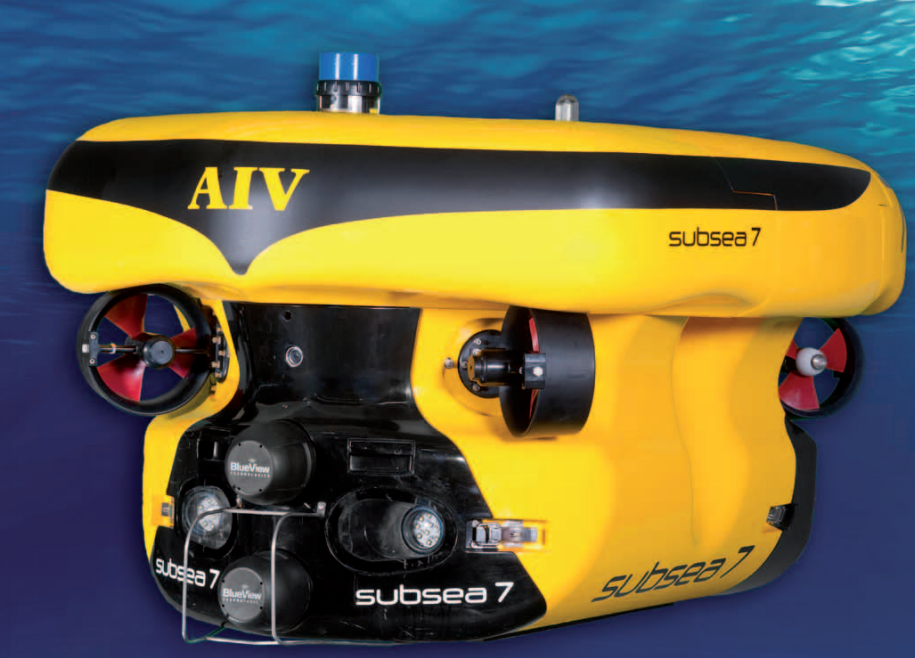
\includegraphics[width=0.48\textwidth]{subsea7AIV}
	\end{center}
	
	\caption{Subsea 7's AIV. This is the first commercial autonomous inspection vehicle for subsea operations \cite{pressAIV}}
	%\vspace{-20pt}
\end{wrapfigure}

Subsea maintenance is perhaps the field that have seen the greatest advancements in autonomous inspection and maintenance. As offshore installations are moved to the seabed, maintenance and inspection has become a significant challenge. This has resulted in a widespread use of \acp{ROV}. Recent developments in other fields, e.g. computer vision, human-robot collaboration and machine learning, has resulted in new \acp{AIV} and \acp{AUV} capable of performing inspection and simple maintenance tasks autonomously\cite{subseaAIV}\cite{Ridao2015227}. A driving factor behind the transition from \acp{ROV} to \acp{AUV} is cost reduction through increased offshore campaign efficiency.

\subsection{Disaster Response}

\begin{wrapfigure}{r}{0.5\textwidth}
	%\vspace{-20pt}
	\begin{center}
		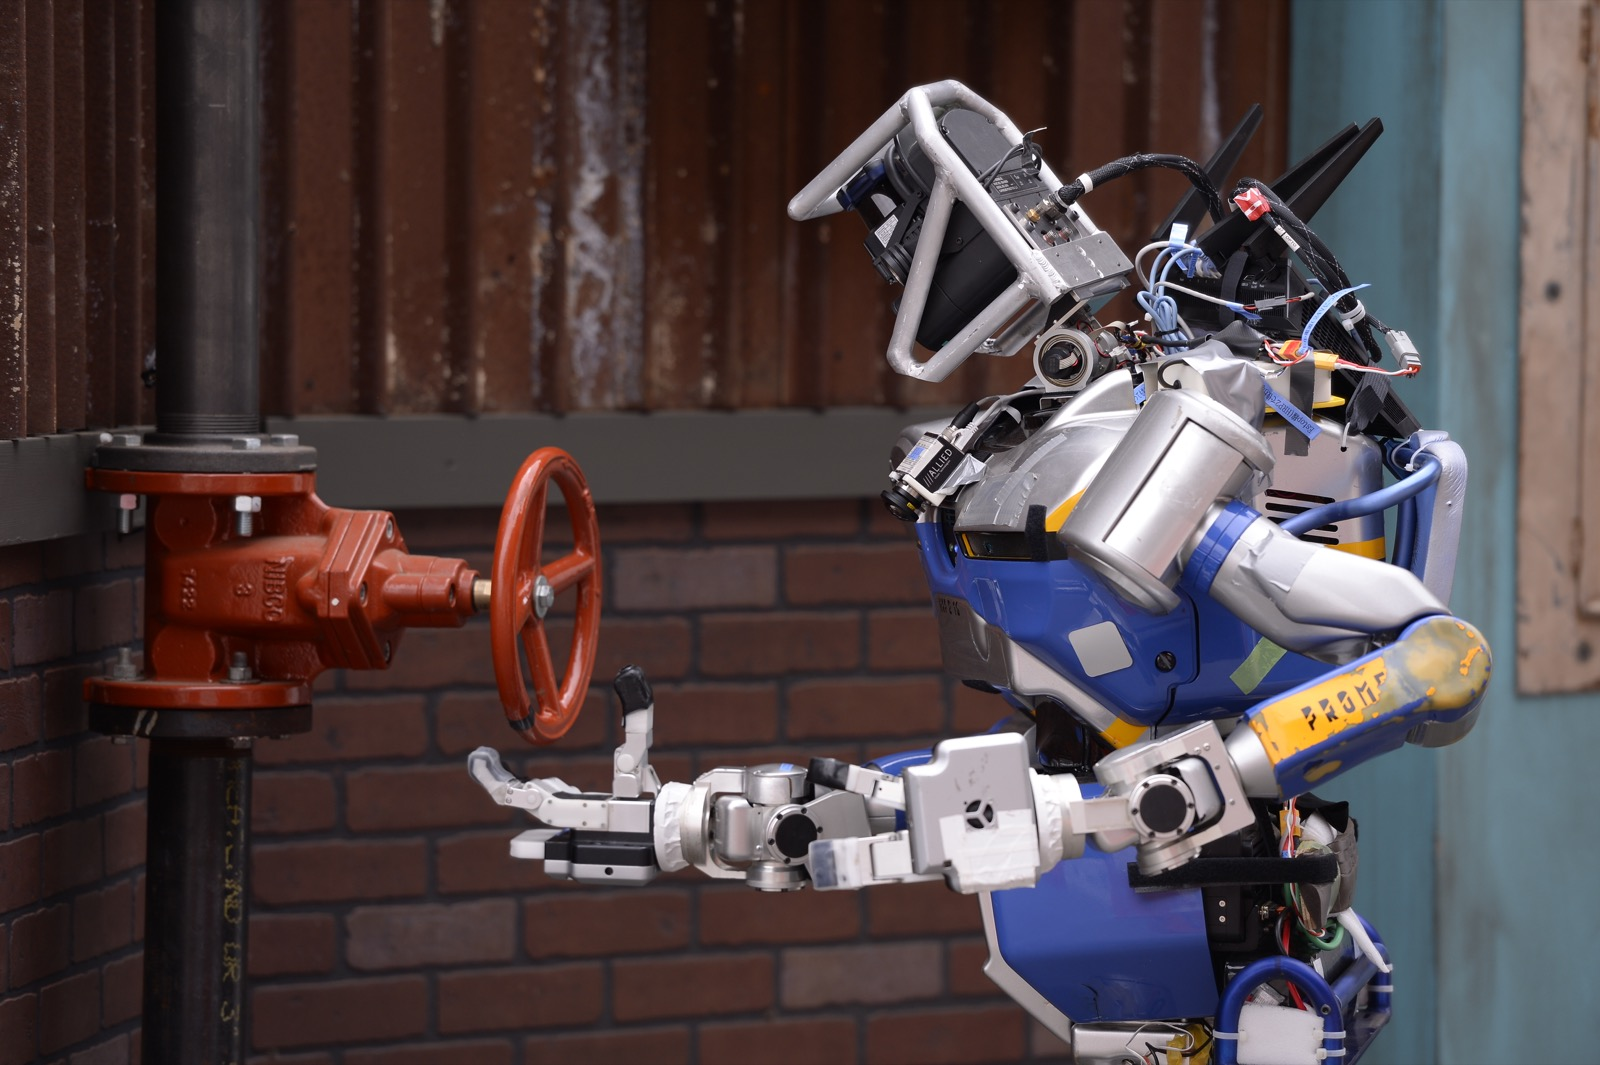
\includegraphics[width=0.48\textwidth]{HRP2_valve}
	\end{center}
	
	\caption{Team HRP2-Tokyo's robot turning a valve during DARPA Robotics Challenge 2015 (Image credits: DARPA Robotics Challenge)}
	%\vspace{-20pt}
\end{wrapfigure}

Robots in disaster response, relief and recovery solve many of the same problems faced by maintenance robots. Disasters, such as the tsunami which struck Japan in 2011, proved that much work needs to be done, both in terms of technical capabilities and logistical issues related to deployment and response times. The tsunami resulted in three core meltdowns at the Fukushima Daiichi Nuclear Power plant.

Many of the robots which were deployed at the Fukushima Power Plant were already ageing, and the operators had to receive training before deployment, thus increasing the response time\cite{doi:10.1108/01439911211249715}. A paper from Japan Atomic Energy Agency\cite{doi:10.1108/01439911211249715} highlights how the lack of stakeholder involvement could have been the cause of long response times. The same paper points out that the robots were developed for the sake of development, and not with emergency response as the main purpose\cite{doi:10.1108/01439911211249715}. 

\ac{DRC}\cite{DRC} was launched in response to the Fukushima disaster of 2011. The purpose of the competition is to accelerate innovation, research and development in robotics for disaster response in cases where humans cannot operate. Some of the tasks the competitors faces in 2015 include valve turning, traversing rubble and driving a vehicle through a course before egressing out of the vehicle.

\subsection{Topside Offshore and Onshore Robotic Maintenance}

\begin{wrapfigure}{l}{0.45\textwidth}
	%\vspace{-20pt}
	\begin{center}
		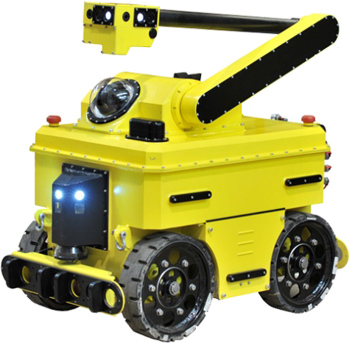
\includegraphics[width=0.42\textwidth]{sensabot}
	\end{center}
	
	\caption{An early version of the maintenance robot ''Sensabot'', developed by National Robotic Engineering Center (NREC) (Image credits: NREC)}
	\vspace{-20pt}
\end{wrapfigure} 

Today, autonomous and teleoperated inspection and maintenance is usually only found at subsea installations. Topside installations on the other hand are still maintained and inspected manually, with some notable exceptions. Small \acp{UAV} or \acp{RPAS} have become commonplace and accessible to all over the last decade. There are currently \ac{RPAS} systems which are being used for visual inspection of inaccessible structural parts such as flare stacks or the exterior of oil rigs.

Some notable contributors to the field of robotic maintenance for \ac{OG} include ABB, \ac{Fraunhofer IPA}, Sintef ICT\cite{sintef_robot_consept} and NREC  at  Carnegie
Mellon University. 

NRECs contribution, Sensabot, is a remotely operated inspection robot designed for harsh and remote environments\cite{deploymentsensabot}. It is not designed to be autonomous, but rather as a tool to move personnel from hazardous environments to safe remote control rooms. Sensabot mark II will be certified for zone 1 explosive environments. This year (2016), the plan is to test the robot on site at the Kashagan field in Kazakhstan\cite{peerless2016robot}.

\ac{Fraunhofer IPA}\footnote{http://www.ipa.fraunhofer.de/en.html} has developed a robot, called \ac{MIMROex}. \ac{MIMROex} has capabilities which are quite similar to the prototype used during the work on this thesis. \ac{MIMROex} is equipped with a camera for visual inspections as well as microphones, vibration and sensors for fire and gas detection. It is also certifiable in accordance with the explosion protection standard IEC 60079\cite{MIMROex}. \ac{Fraunhofer IPA} put great emphasis on field testing on actual offshore installations.

Both ABB and SINTEF ICT has developed lab facilities to test various concepts for robotic maintenance. Both facilities use non-mobile robots which utilize a rich set of inspection and manipulation tools, as well as \ac{HMI} equipment for remote operation and control. The two research communities differ in that ABB has tested their solutions in real environments, which subjects their solution to ATEX requirements and an extensive risk management regime\cite{StepwiseApproachToRobotics}. SINTEF has a long list of contributui

Another effort towards robotic maintenance is the ARGOS challenge (Autonomous Robot for Gas and Oil Sites). The purpose of the challenge is to promote innovation, understanding and awareness towards robotic maintenance of \ac{OG} sites in harsh environments\cite{ARGOS}.